%%%%%%%%%%%%%%%%%%%%%%%%%%%%%%%%%%%%%%%
% Header                              %
%%%%%%%%%%%%%%%%%%%%%%%%%%%%%%%%%%%%%%%
% 
% Revisions: 2017-12-12 Martin Raedel <martin.raedel@dlr.de>
%                       Initial draft
%               
% Contact:   Martin Raedel,  martin.raedel@dlr.de
%            DLR Composite Structures and Adaptive Systems
%          
%                                 __/|__
%                                /_/_/_/  
%            www.dlr.de/fa/en      |/ DLR
% 
%%%%%%%%%%%%%%%%%%%%%%%%%%%%%%%%%%%%%%%
% Content                             %
%%%%%%%%%%%%%%%%%%%%%%%%%%%%%%%%%%%%%%%

\begin{tikzpicture}[
  every node/.style={font=\figurefontsize},
  %inner sep=0pt,
]
  % External figure
  \node[anchor=south west,inner sep=0] (image) at (0,0) {
    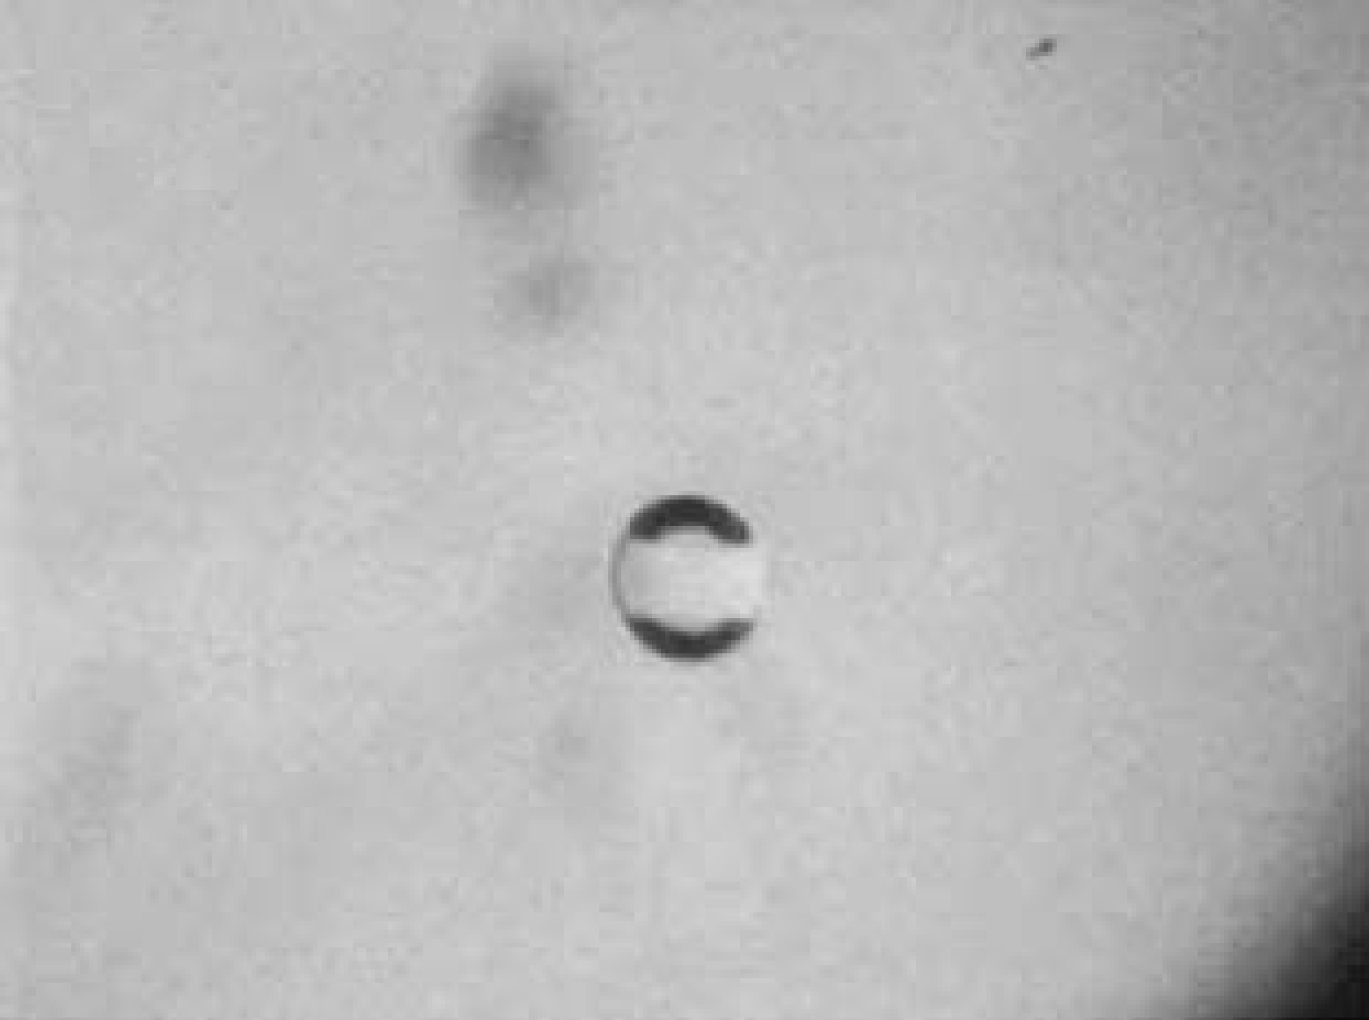
\includegraphics[angle=90,origin=c,width=\figwidth,height=\figheight,keepaspectratio]{Exp_Fibre_Cho2006_IV_woLabels.png}
  };
  % Figure scope
  \begin{scope}[
    x={(image.south east)},
    y={(image.north west)},
  ]
    
    % Load arrows
    \foreach \y in {0,1,...,\numarrows} {\draw[-latex] (-0.025,\y/\numarrows) -- (-0.15,\y/\numarrows) coordinate (loadarrowleft\y);}
    \foreach \y in {0,1,...,\numarrows} {\draw[-latex] ( 1.025,\y/\numarrows) -- ( 1.15,\y/\numarrows) coordinate (loadarrowright\y);}
    
    % Help grid and labels
    %\pic{myimagegrid};
  \end{scope}
\end{tikzpicture}